\chapter{\selectlanguage{greek}Κώδικες Επανάληψης-Συσσώρευσης \en{(repeat - accumulate, RA)}}
\externaldocument{chapter1.tex}
\externaldocument{chapter2.tex}

Στο κεφάλαιο αυτό, παρουσιάζονται οι κώδικες Επανάληψης-Συσσώρευσης \en{(repeat - accumulate, RA)}, η μελέτη της επίδοσης των οποίων αποτελεί και το αντικείμενο της παρούσας εργασίας.

Οι \en{RA} αποτελούν τους πρώτους κώδικες που βασίζονται σε συσσωρευτές και εφευρέθηκαν από τους \en{D. Divsalar} κ .ά. \cite{divsalar1998coding}. Ενώ έχουν απλή δομή, δακρίνονται από καλές επιδόσεις και πρακτική κωδικοποίηση, με μοναδικό μειονέκτημα ότι υστερούν από άποψη επιδόσεων στους χαμηλούς ρυθμούς (1/2 ή χαμηλότερου). Πλέον, χρησιμοποιούνται ήδη σε αρκετά πρότυπα τηλεπικοινωνιών (\en{DVB-S2, IEEE802.16}). Διακρίνονται ως μια ειδική κλάση των \textit{σειριακά αλυσιδωτών} κωδίκων (\en{serially concatenated codes - SC}), στους οποίους ο εξωτερικός κώδικας είναι ένας επαναληπτικός κώδικας ρυθμού $1/q$ και ο εσωτερικός είναι ένας συνελικτικός κώδικας γεννήτορα $\frac{1}{1+D}$, ο οποίος δίνει το $mod-2$ άθροισμα του \en{bit} εισόδου με το προηγούμενο \en{bit} εξόδου. Παράγει δηλαδή το άθροισμα όλων των παρελθουσών εισόδων και για το λόγο αυτό καλείται και \textit{συσσωρρευτής} (\en{accumulator}), στοιχείο που δίνει στους \en{RA} το όνομά τους.

\begin{figure}[h]
\center{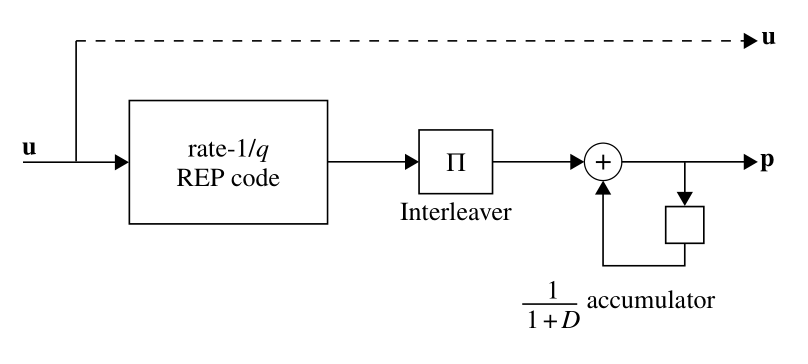
\includegraphics[width=0.65\linewidth]{figures/Ra_scheme.png}}
\caption{Μπλοκ διάγραμμα ενός \en{RA} κώδικα}
\label{fig:RA scheme graph}
\end{figure}

Οι \en{RA} που μεταδίδουν τα \en{bits} πληροφορίας αυτούσια λέγονται συστηματικοί. Ένα σχηματικό διάγραμα ενός συστηματικόυ \en{RA} κώδικα, φαίνεται στο Σχήμα \ref{fig:RA scheme graph}. Η αποκωδικοποίησή τους μπορεί να αντιμετωπισθεί είτε ως σειριακή \en{turbo}, είτε ως \en{LDPC}, τακτική που είναι και η πιο διαδεδομένη \cite{ryan2009channel}.


Στη συνέχεια του κεφαλαίου παρουσιάζονται συνοπτικά οι κώδικες που μπορούν να πλησιάσουν το θεωρητικό όριο χωρητικότητας \en{Shannon} (Θεώρημα \ref{theorem:shannon}), διατηρώντας παράλληλα τη δυνατότητα πρακτικής κωδικοποίησης και αποκωδικοποίησης. Αφού γίνει μια σύντομη αναφορά στη σχέση χωρητικότητας και σηματοθορυβικής σχέσης (\en{SNR}), παρουσιάζονται οι τρόποι θεώρησης των \en{RA}, είτε ως \en{turbo}, είτε ως \en{LDPC}. Κατόπιν αφού αναλυθεί ο τρόπος κωδικοποίησης των \en{LDPC} (ως ο πιο συχνός τρόπος θεώρησης των \en{RA}), δίνεται πλήρως το \en{coding scheme} των \en{RA}, που δίνει και τη βάση πάνω στην οποία στηρίζεται η προσομοίωση που έγινε και θα αναλυθεί στο Κεφάλαιο 4.

\section{Κώδικες που πλησιάζουν τη χωρητικότητα}

Μέχρι και πολύ πρόσφατα, οι κώδικες που μπορούσαν να λειτουργήσουν κοντά στο θεωρητικό όριο χωρητικότητας που προέβλεπε το θεώρημα \en{Shannon}, ήταν κυρίως μη πρακτικοί κώδικες. Με την ανακάλυψη των \en{turbo} κωδίκων και την επανανακάλυψη των \en{LDPC} τη δεκαετία του '90, έγινε δυνατό να αποδειχθεί η ικανότητα λειτουργίας τους κοντά στη χωρητικότητα, με πρακτικά υλοποιήσιμους κωδικοποιητές-αποκωδικοποιητές σε σχετικά χαμηλά \en{bit error rates (BERs)}, όσον αφορά το κανάλι \en{AWGN}. 

Παρ'όλο που η θεωρητική επίτευξη του ορίου χωρητικότητας απαιτεί κώδικες με άπειρο μήκος, στην πράξη αρκεί το μήκος του κώδικα να είναι αρκετά μεγάλο (π.χ. της τάξης των μερικών δεκάδων χιλιάδων). Η σχεδίαση τέτοιων κωδίκων χαρακτηρίζεται από 2 βασικά στοιχεία:
\begin{itemize}
\item Χρήση κωδίκων αποτελούμενων από απλά μέρη, συνενωμένα με τρόπο που να παράγεται μια ψευδο-τυχαία κατανομή βαρών και,
\item Χρήση υποβέλτιστων επαναληπτικών αλγορίθμων αποκωδικοποίησης με ανταλλαγή \en{soft} πληροφορίας, των οποίων η πολυπλοκότητα αυξάνει γραμμικά με την αύξηση του μήκους κώδικα.
\end{itemize}

Μπορεί επίσης να δοθεί και ο παρακάτω ορισμός των κωδίκων που πλησιάζουν τη χωρητικότητα:
\begin{definition}\en{Capacity-approaching} κώδικες

Έστω μια ακολουθία από δυαδικούς γραμμικούς κώδικες $\left( C_m \right)$, ρυθμού $R_m$ και για κάθε κώδικα, οι κωδικές λέξεις μεταδίδονται ισοπίθανα μέσω ενός καναλιού με χωρητικότητα $C$. Η ακολουθία επιτυγχάνει κλάσμα $1-\epsilon$ της χωρητικότητας του καναλιού αν $\lim_{m\to \infty}R_m\geq\left(1-\epsilon\right)\cdot C$ και υπάρχει αλγόριθμος αποκωδικοποίησης για τον οποίο η πιθανότητα εσφαλμένου \en{bit} του κώδικα $C_m$ τείνει στο μηδέν, όταν $m\to \infty$ \cite{pfister2005capacity}.
\label{def:capacity approaching codes}
\end{definition}

Δύο πολύ γνωστές κλάσεις \en{capacity-approaching} κωδίκων είναι οι εξής: οι \en{turbo} ή \en{turbo-like} κώδικες, οι οποίοι συνίστανται από συνελικτικούς συστατικούς κώδικες (\en{component codes}) και οι κώδικες Ελέγχου Ισοτιμίας Χαμηλής Πυκνότητας (\en{Low Density Parity Check - LDPC}).

\begin{figure}[h]
\center{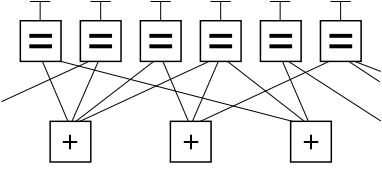
\includegraphics[width=0.65\linewidth]{figures/LDPC_factor_graph.png}}
\caption{Μέρος του γραφήματος παραγόντων ενός \en{LDPC} κώδικα}
\label{fig:LDPC factor graph}
\end{figure}

Και οι δύο κατηγορίες που αναφέρθηκαν χαρακτηρίζονται ως \textit{Κώδικες σε Γραφήματα} (\en{Codes on Graphs}), διότι αναπαρίστανται από \textit{γραφήματα παραγόντων} (\en{factor graphs}) πάνω στα οποία εκτελείται ο αλγόριθμος για την επαναληπτική αποκωδικοποίησή τους. Στο Σχήμα \ref{fig:LDPC factor graph} παραθέτουμε μέρος του γραφήματος ενός \en{LDPC} κώδικα \cite{ryan2009channel}, \cite{johnson2009iterative}, \cite{codes2009guest}.

\subsection{Η χωρητικότητα ως \en{SNR}}

Σε αυτό το σημείο θα γίνει μια σύντομη αναφορά στη σχέση που συνδέει τη χωρητικότητα ενός καναλιού με τη σηματοθορυβική σχέση \en{SNR} που το χαρακτηρίζει.

\begin{figure}[h]
\center{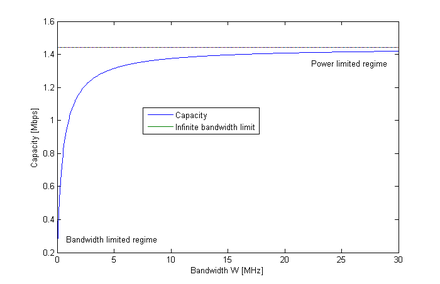
\includegraphics[width=0.55\linewidth]{figures/Channel_capacity.png}}
\caption{Χωρητικότητα \en{AWGN} καναλιού}
\label{fig:Channel capacity}
\end{figure}

Έστω τηλεπικοινωνιακό σύστημα που εισάγει \en{AWGN} θόρυβο. Η χωρητικότητα καναλιού αποδεικνύεται ότι δίνεται από την παρακάτω εξίσωση:

\begin{equation}
C=\frac{1}{2}\log_2(1+SNR)\;\;\;\text{\en{bit}/μετάδοση}
\label{eq:capacity vs SNR}
\end{equation}

Από την παραπάνω σχέση φαίνεται ότι η χωρητικότητα εξαρτάται μόνο από το \en{SNR}. Από εδώ και στο εξής, ως χωρητικότητα θα εννοούμε το ελάχιστο \en{SNR} που απαιτείται (συνήθως ως $E_b/N_0$) για την επίτευξη οσοδήποτε αξιόπιστης επικοινωνίας με δεδομένο ρυθμό $C$, όπως φαίνεται και από το Σχήμα \ref{fig:Channel capacity}.

\section{\en{RA} ως \en{turbo}}

Σε αυτή την παράγραφο, θα γίνει μια σύντομη αναφορά στους κώδικες \en{turbo}, την αποκωδικοποίησή τους, καθώς και την δυνατότητα των \en{RA} να χαρακτηριστούν ως τέτοιοι.

\subsection{Κώδικες \en{turbo}}

Οι κώδικες \en{turbo} ανακαλύφθηκαν από τους \en{Berrou, Glavieux} και \en{Thitimajshima} \cite{berrou1993near} το 1993 και αποτέλεσαν ριζοσπαστική προσέγγιση της κωδικοποίησης για διόρθωση σφαλμάτων. Αποτελούνται από τον παράλληλο συνδυασμό δύο συνελικτικών κωδίκων, οι οποίοι κατά την αποκωδικοποίηση διαμοιράζουν πληροφορία μεταξύ των αντίστοιχων αποκωδικοποιητών. Αναφέρεται πως ο κωδικοποιητής χρησιμοποιεί συνελικτικούς κωδικοποιητές \cite{hagenauer1996iterative}, ενώ ο αποκωδικοποιητής χρησιμοποιεί \en{BCJR} αποκωδικοποιητές \cite{abrantes2004bcjr}.


\begin{figure}[h]
    \centering
    \begin{minipage}{0.7\textwidth}
        \centering
        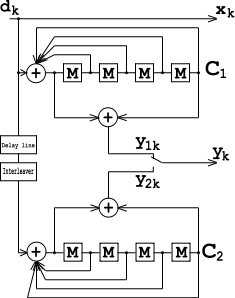
\includegraphics[width=0.9\textwidth]{figures/Turbo_encoder.png}
        \caption{Κωδικοποιητής \en{turbo}}
    \end{minipage}\hfill
    \begin{minipage}{0.7\textwidth}
        \centering
        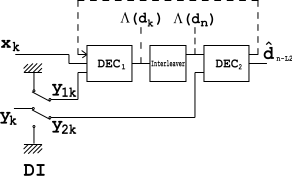
\includegraphics[width=0.9\textwidth]{figures/Turbo_decoder.png}
        \caption{Αποκωδικοποιητής \en{turbo}}
    \end{minipage}
\end{figure}

Ο κωδικοποιητής \en{turbo} περιέχει έναν \textit{αναδιατάκτη} (\en{interleaver}), ο ρόλος του οποίου είναι να μεταθέτει κωδικές λέξεις μικρού βάρους από τον ένα κωδικοποιητή σε κωδικές λέξεις μεγάλου βάρους στον άλλο. Ο αναδιατάκτης αυτός διαθέτει ψευδοτυχαία χαρακτηριστικά.

Η αποκωδικοποίηση στηρίζεται στην ανταλλαγή \en{soft} πληροφορίας μεταξύ δύο συστατικών αποκωδικοποιητών. Η πληροφορία αυτή έχει τη μορφή λογαριθμικού λόγου πιθανοτήτων (\en{log-likelihood ratio, LLR}) για καθένα από τα \en{bits} πληροφορίας. \cite{berrou1993near}.

\subsection{Κωδικοποίηση \en{RA}}

Το συνολικό \en{coding scheme} των \en{RA} που προσομοιώθηκε θα αναλυθεί στη συνέχεια του κεφαλαίου. Ωστόσο, η αποκωδικοποίηση τους μπορεί να βασιστεί στην \en{turbo} αποκωδικοποίηση των \en{SC}, όπου, όπως αναφέρθηκε ήδη, ο εξωτερικός κώδικας είναι \en{repetition} και ο εσωτερικός είναι ο \en{accumulator}. Για τους συστηματικούς \en{RA} κώδικες που περιέχουν συνδυαστή, ο εσωτερικός κώδικας είναι συνδυαστικός αποκωδικοποιητής συνδυαστή-συσσωρευτή (\en{accumulator-combiner - AC}) και ο \en{REP} αποκωδικοποιητής έχει ως είσοδο τα \en{LLRs} από το κανάλι \cite{johnson2009iterative}.

\begin{figure}[h]
\center{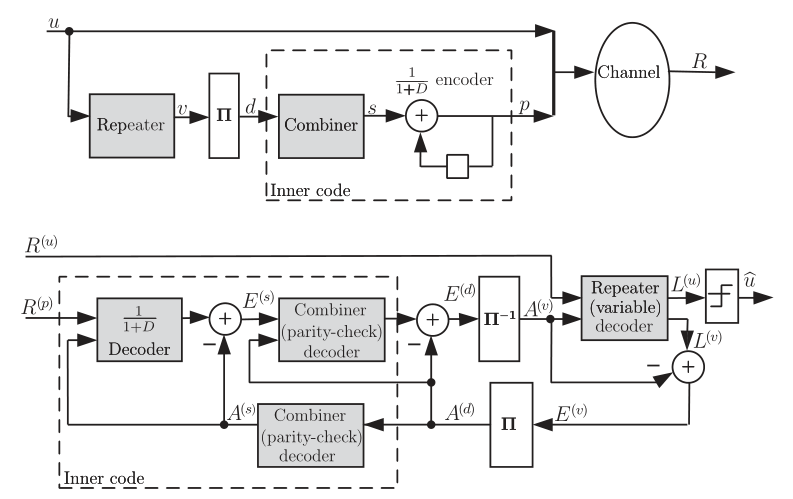
\includegraphics[width=0.85\linewidth]{figures/systematic_RA.png}}
\caption{Κωδικοποιητής / \en{turbo} αποκωδικοποιητής συστηματικού \en{RA}}
\label{fig:enc/turbo dec of systematic RA}
\end{figure}

Στο Σχήμα \ref{fig:enc/turbo dec of systematic RA}, φαίνεται η κωδικοποίηση και αποκωδικοποίηση \en{turbo} ενός \en{RA} κώδικα, βάσει της \textit{αρχής \en{turbo}} (\en{turbo principle}) \cite{hagenauer2003turbo}. Σε κάθε επανάληψη της αποκωδικοποίησης, ο \en{REP} αποκωδικοποιητής λαμβάνει \en{LLRs} από το κανάλι αναφορικά με τα κωδικά \en{bits} και στις επόμενες επαναλήψεις, ως επιπλέον, \en{a priori} πληροφορία τα \en{LLRs} εξωγενούς πληροφορίας από τον \en{AC} αποκωδικοποιητή.

Στο επόμενο βήμα ο \en{REP} αποκωδικοποιητής υπολογίζει τα \en{LLRs} εξόδου. Η εξωγενής πληροφορία από τον \en{REP} αποκωδικοποιητή, παρεμβάλλεται από τον \en{interleaver} για την παραγωγή \en{a-priori LLRs} στον \en{AC} αποκωδικοποιητή. Στην τελική επανάληψη, λαμβάνεται απόφαση για τα \en{bits} πληροφορίας από τα τελικά \en{LLRs} που εξάγει ο \en{REP} αποκωδικοποιητής. Ο αλγόριθμος τελειώνει μετά από ένα προκαθορισμένο αριθμό $I_{max}$ επαναλήψεων. Το \en{block} διάγραμμα διαμόρφωσης της κωδικής λέξης ενός \en{RA} κώδικα, δόθηκε ήδη στο Σχήμα \ref{fig:RA scheme graph}. Τα \en{bits} πληροφορίας αντιγράφονται $q$ φορές, περνούν από τον αναδιατάκτη, ομαδοποιούνται μέσω $mod-2$ πρόσθεσης σε \en{block} μήκους $a$ και τέλος περνούν από ένα συνελικτικό κωδικοποιητή μνήμης -1.

Πιο συγκεκριμένα, το μήνυμα πληροφορίας μήκους $k$, $\mathbf{u}=\left(u_0,u_1,\cdots,u_{k-1}\right)$, μετά την έξοδο από τον επαναληπτικό κωδικοποιητή, έχει τη μορφή:

\begin{equation}
\begin{split}
\mathbf{c} &= \left[c_1, c_2, \cdots, c_{qk} \right] \\
&= (\underbrace{u_0,u_0,\cdots,u_0}_q, \; \underbrace{u_1,u_1,\cdots,u_1,}_q, \; \cdots, \; \underbrace{u_{k-1},u_{k-1},\cdots,u_{k-1}}_q)
\end{split}
\end{equation}
, όπου $c_i=u_{f(i)}$ με $f(i)=\lceil i/q \rceil$ και $\lceil x \rceil$ τον αμέσως μεγαλύτερο ακέραιο από το $x$.

Κατόπιν, κατά την έξοδο από τον αναδιατάκτη $\Pi=[\pi_1,\pi_2,\cdots,\pi_{qk}]$, διαμορφώνεται μια μετάθεση της ακολουθίας $\mathbf{c}$ ως εξής:

\begin{equation*}
\mathbf{d} = \left[d_1, d_2, \cdots, d_{qk} \right] = [c_{\pi_1}, c_{\pi_2}, \cdots, c_{\pi_{qk}}]
\end{equation*}

Ο συνδυαστής λαμβάνει την έξοδο του αναδιατάκτη, προσθέτει ($mod-2$) και ομαδοποιεί τα \en{bits} σε \en{block} μήκους $a$. Τα \en{bits} της ακολουθίας εξόδου του συνδυαστή $\mathbf{s}$, δίνονται από την εξίσωση:

\begin{equation}
s_i=d_{a(i-1)+1}\oplus d_{a(i-1)+2} \oplus \cdots \oplus d_{ai}, \;\;\; i=1,2,\cdots,m\;\;m=kq/a
\label{eq:combiner equation}
\end{equation}

Στην έξοδο του συσσωρευτή, τα \en{parity bits} θα δίνονται από την εξίσωση:

\begin{equation}
\begin{aligned}
p_0 & = 0 \\ 
p_i & =p_{i-1}\oplus s_i\;\;\; i=1,2,\cdots,m
\end{aligned}
\label{eq:accumulator equation}
\end{equation}

Από την εξίσωση \ref{eq:accumulator equation}, προκύπτει πως η κωδική λέξη του συστηματικού \en{RA} κώδικα, έχει τη μορφή $\mathbf{v}=[u_0, u_1,\cdots,u_{k-1},p_1,p_2,\cdots,p_m]$, οπότε το μήκος του κώδικα προκύπτει $n=k(1+q/a)$ και ο ρυθμός $R=a/(a+q)$ \cite{johnson2009iterative}.



\section{\en{RA} ως \en{LDPC}}

Οι κώδικες \en{LDPC} παρουσιάστηκαν για πρώτη φορά το 1962 από τον \en{R. G. Gallager} στη διδακτορική του διατριβή \cite{gallager1962low} και αποτελούν κώδικες διόρθωσης σφαλμάτων που ορίζονται από αραιό πίνακα ελέγχου ισοτιμίας. Παρά το ότι αποτελούν \en{capacity-approaching} κώδικες εγκαταλείφθηκαν για περίπου 30 χρόνια, με εξαίρεση τη δουλειά του \en{Tanner} \cite{tanner1981recursive} που εισήγαγε και τη γραφική αναπαράστασή τους, μέσω του γραφήματος \en{Tanner}, λόγω περιορισμών στην τεχνική τους υλοποίηση και επανανακαλύφθηκαν το 1996 από τους \en{Mackay} κ.α. \cite{mackay1996near}. Tο κύριο χαρακτηριστικό τους, η χαμηλή πυκνότητα του πίνακα $\mathbf{H}$, είναι και αυτό που κάνει τους \en{LDPC} να επιδέχονται διάφορους αλγόριθμους επαναληπτικής αποκωδικοποίησης (\en{iterative decoding}). Παρ’ότι οι αλγόριθμοι επαναληπτικής αποκωδικοποίησης έχουν μη-βέλτιστη απόδοση, μπορούν να έχουν απόδοση που χαρακτηρίζεται “σχεδόν” βέλτιστη (\en{near-optimal}), σε εφαρμογές/\en{error-rates} ενδιαφέροντος. Πρόσφατα αποδείχτηκε από τους \en{Chung, Richardson} κ.α. η δυνατότητα των \en{LDPC} προσέγγισης του θεωρητικού ορίου \en{Shannon} κατά $0.0045\;dB$ \cite{chung2001design}.

Κάθε γραμμικός κώδικας έχει αναπαράσταση μέσω πίνακα ελέγχου-ισοτιμίας, ωστόσο για να είναι \enquote*{αραιή} η αναπαράσταση πρέπει να πληρούνται ορισμένα κριτήρια. Ένας $m\times n$ πίνακας καλείται αραιός αν το ποσό από άσσους (1) στις γραμμές και στις στήλες του, το βάρος γραμμών ($w_r$) και στηλών ($w_c$), είναι πολύ μικρότερο από τις διαστάσεις του ($w_r\ll n$, $w_c\ll m$). Πρακτικά, θεωρείται πως αν λιγότερο από $1\%$ των στοιχείων του πίνακα είναι άσσοι, τότε είναι αραιός. Αν το βάρος γραμμών και στηλών είναι σταθερό ο κώδικας \en{LDPC} λέγεται ομαλός, ενώ σε αντίθετη περίπτωση λέγεται ανώμαλος \cite{ta2013tutorial}.

Γενικά, εκτός από την απαίτηση να είναι ο πίνακας $\mathbf{H}$ αραιός, οι \en{LDPC} δε διαφέρουν από τους μπλοκ κώδικες. Ωστόσο, η εύρεση ενός αραιού πίνακα ελέγχου ισοτιμίας για ένα δεδομένο μπλοκ κώδικα αποτελεί δύσκολη διαδικασία και της κατασκευής των \en{LDPC} προηγείται η κατασκευή του πίνακα $\mathbf{H}$ και ακολουθεί η σχεδίαση του κωδικοποιητή. Οι \en{LDPC} αποκωδικοποιούνται επαναληπτικά, κάνοντας χρήση γραφικής αναπαράστασης του πίνακα ελέγχου ισοτιμίας.

Έχει διαπιστωθεί πως και οι \en{RA} και οι  \en{LDPC} ενέχουν πλεονέκτημα σε σχέση με τους \en{turbo} κώδικες, καθώς προσφέρουν μια πιο ευέλικτη δομή, κάτι που με τη σειρά του προσφέρει περισσότερους βαθμούς ελευθερίας στην επιλογή των παραμέτρων για δεδομένο κριτήριο σχεδίασης \cite{johnson2009iterative}.

\subsection{Κωδικοποίηση \en{LDPC}}

Όπως αναφέρθηκε στο Κεφάλαιο 2, οι γραμμικοί μπλοκ κώδικες αποτυπώνουν το μήνυμα πληροφορίας $\mathbf{u}$ στην κωδική λέξη $\mathbf{v}$ κάνοντας χρήση της εξίσωσης \ref{eq:check equation}, για δοσμένο γεννήτορα πίνακα $\mathbf{G}$. Γενικά, όπως έχει επίσης αναφερθεί και στο Κεφάλαιο 2, ο πίνακας $\mathbf{G}$ ενός κώδικα δίνεται από το \en{null-space} του -αραιού για τους \en{LDPC}- πίνακα $\mathbf{H}$. Συνεπώς είναι απίθανο να είναι και ο ίδιος αραιός, κάτι που θα οδηγούσε σε κέρδος ως προς το χρόνο κωδικοποίησης (ως προς το μήκος του κώδικα). Προκύπτει επομένως πως, η κωδικοποίηση ενός \en{LDPC} με βάση την εξίσωση \ref{eq:check equation} γίνεται σε τετραγωνικό χρόνο ως προς το μήκος κώδικα. Σημειώνεται πως έχουν γίνει διάφορες προσπάθειες προς την κατεύθυνση της μείωσης του χρόνου αυτού. Η πιο εξέχουσα από αυτές είναι η κωδικοποίηση \en{RA} \cite{ta2013tutorial}.

\subsection{Κωδικοποίηση \en{RA}}

Ο πίνακας $\mathbf{H}$ των \en{RA} κωδίκων έχει την ακόλουθη ειδική μορφή: 

\begin{equation}
\mathbf{Η} = \left[Η_1\;Η_2\right]
\label{eq:form of RA parity matrix}
\end{equation}

Έχοντας τον υποπίνακα $H_2$ στη μορφή \ref{eq:parity check submatrix form} παρατηρούμε ότι το πρώτο \en{parity-check bit} υπολογίζεται από μια υποομάδα των \en{bits} πληροφορίας που ορίζει η πρώτη γραμμή του υποπίνακα $H_1$. Κατόπιν, το δεύτερο \en{parity-check bit} υπολογίζεται από το άρτι υπολογισθέν \en{bit} ελέγχου ισοτιμίας συν μια υποομάδα \en{bits} ληροφορίας που ορίζει η δεύτερη γραμμή του υποπίνακα $H_1$. Έτσι, η διαδικασία της κωδικοποίησης καθίσταται γραμμικού χρόνου. Αντιλαμβανόμαστε ότι ο υποπίνακας $H_2$ αντιστοιχεί στη λειτουργία του συσσωρευτή, ενώ ο $H_1$ στις λειτουργίες του επαναληπτικού κώδικα, του αναδιατάκτη και του συνδυαστή.

\begin{equation}
\mathbf{H}_2=\begin{bmatrix}
1 & 0 & 0 &  & 0 & 0 & 0 \\
1 & 1 & 0 & \cdots & 0 & 0 & 0 \\
0 & 1 & 1 & \;\; & 0 & 0 & 0 \\
  & \vdots & & \ddots & & \vdots & \\
0 & 0 & 0 &  & 1 & 0 & 0 \\
0 & 0 & 0 & \cdots & 1 & 1 & 0 \\
0 & 0 & 0 &  & 0 & 1 & 1 \\
\end{bmatrix}
\label{eq:parity check submatrix form}
\end{equation}


\subsection{Αποκωδικοποίηση \en{RA}}

Αναφέρθηκε ήδη η δυνατότητα των \en{RA} κωδίκων για \en{turbo} αποκωδικοποίηση. Ωστόσο, στο πλαίσιο της συγκεκριμένης εργασίας, μελετάται η δυνατότητα για αποκωδικοποίηση ως \en{LDPC}, χρησιμοποιώντας τον αλγόριθμο \en{\textit{Sum-Product} (Sum-Product algorithm, SPA)}.

Ο αλγόριθμος παρουσιάστηκε από τον \en{Gallager} μαζί με τους κώδικες \en{LDPC}. Χαρακτηρίζεται από \en{near-optimal} επίδοση αποκωδικοποίησης καθώς και από καθολικότητα για τα διάφορα κανάλια χωρίς μνήμη (\en{BEC, BSC, BI-AWGN}, κ.λ.π.), συνεπώς η ανάπτυξή του είναι γενική. Το κριτήριο βέλτιστης ανάπτυξης του αλγορίθμου, είναι ο υπολογισμός της μέγιστης εκ των υστέρων (\en{maximum a posteriori - MAP}) πιθανότητας. Υπολογίζεται δηλαδή η (εκ των υστέρων) πιθανότητα για την τιμή κάθε συγκεκριμένου \en{bit} της κωδικής λέξης $\mathbf{v}$, με δεδομένο το ληφθέν διάνυσμα $\mathbf{r}$.

\subsubsection{Το γράφημα \en{Tanner}}

Το γράφημα \en{Tanner} ενός \en{LDPC} κώδικα \cite{tanner1981recursive}, είναι ένα \textit{διμερές} γράφημα (\en{bipartite graph}) το οποίο δίνει μια πλήρη αναπαράσταση του κώδικα και αποτυπώνει τη λειτουργία των αλγορίθμων αποκωδικοποίησής του. Αποτελείται από δύο διαφορετικού τύπου κόμβους, με τις ακμές του να συνδέουν αποκλειστικά κόμβους του αντίθετου τύπου.

Οι δύο τύποι κόμβων στο γράφημα \en{Tanner} είναι οι \textit{κόμβοι μεταβλητών} (\en{variable nodes, VNs}) και οι \textit{κόμβοι ελέγχου} (\en{check nodes, CNs}). Ο σχηματισμός του γραφήματος \en{Tanner} γίνεται συνδέοντας τον \en{CN} $i$ με τον \en{VN} $j$, αν το στοιχείο $h_{ij}$ του πίνακα $\mathbf{H}$ είναι 1. Παρατηρείται επομένως πως υπάρχουν ακριβώς $m$ \en{CNs}, ένας για κάθε μια εξίσωση ελέγχου και $n$ \en{VNs}, ένας για κάθε κωδικό \en{bit}. Αντίστοιχα οι $m$ γραμμές του $\mathbf{H}$ αντιπροσωπεύουν τις συνδέσεις των \en{CN} και οι $n$ στήλες τις συνδέσεις των \en{VN}. Τέλος, οι $n$-\en{bit} κωδικές λέξεις που αντιπροσωπεύονται από τους \en{VNs}, είναι ακριβώς όλες οι κωδικές λέξεις του κώδικα.

Για τους \en{LDPC} κώδικες, το γράφημα \en{Tanner} αποτελεί σκιαγράφημα της επαναληπτικής αποκωδικοποίησης, καθώς κάθε κόμβος δρα σαν τοπικός επεξεργαστής και κάθε ακμή σα δίαυλος μεταφοράς πληροφορίας, από ένα κόμβο στους γειτονικούς. Η ανταλλασσόμενη πληροφορία είναι πιθανοτική, π.χ. \en{LLRs} \cite{ryan2009channel}.

\subsubsection{Ο \en{Sum-Product} αλγόριθμος για \en{LDPC}}

Η αποκωδικοποίηση του κωδικού \en{bit} $v_j$ απαιτεί τον υπολογισμό της \en{APP} πιθανότητας (για τιμή \en{bit} 1):
\begin{equation*}
\Pr(v_j=1|\mathbf{r})
\end{equation*}
το λόγο \en{APP}
\begin{equation*}
l(v_j|\mathbf{r})\triangleq\frac{\Pr(v_j=0|\mathbf{r})}{\Pr(v_j=1|\mathbf{r})}
\end{equation*}
ή το (σταθερότερο αριθμητικά) λόγο \en{log-APP}, που καλείται επίσης \en{log-likelihood ration (LLR)}:

\begin{equation}
L(v_j|\mathbf{r})\triangleq\log\left(\frac{\Pr(v_j=0|\mathbf{r})}{\Pr(v_j=1|\mathbf{r})}\right)
\label{eq:LLR}
\end{equation}

\begin{figure}[h]
\center{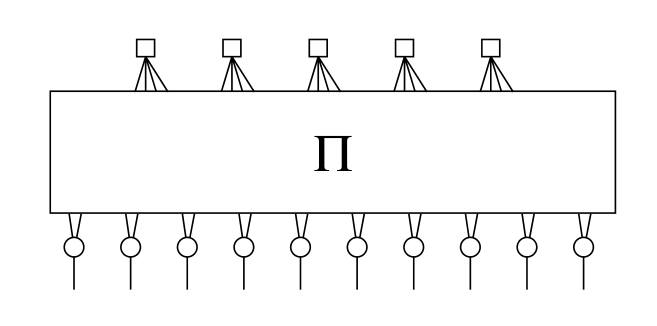
\includegraphics[width=0.6\linewidth]{figures/LDPC_graphical.png}}
\caption{Αναπαράσταση \en{LDPC} ως αλληλουχία από \en{SPC} (επάνω) και \en{REP} (κάτω) κώδικες. Με $\Pi$ συμβολίζεται η αναδιάταξη}
\label{fig:LDPC graphical}
\end{figure}

Ο υπολογισμός της εξίσωσης \ref{eq:LLR} γίνεται εφαρμόζοντας την αρχή \en{turbo} στο γράφημα \en{Tanner}. Με αναφορά το Σχήμα \ref{fig:LDPC graphical}, ο \en{LDPC} μπορεί να θεωρηθεί ως ένα σύνολο από \en{SPC} κώδικες συνδεόμενους μέσω του αναδιατάκτη σε ένα σύνολο \en{REP} κωδίκων. Οι \en{SPC} κώδικες (\en{CNs} στο γράφημα \en{Tanner}) θεωρούνται εξωτερικοί κώδικες, συνεπώς δε συνδέονται στο κανάλι.

Τα Σχήματα \ref{fig:VN}, \ref{fig:CN} αναπαριστούν στιγμιότυπα των \en{REP} και \en{SPC} αποκωδικοποιητών (κόμβοι \en{VN} και \en{CN} αντίστοιχα).

\begin{figure}[h]
    \centering
    \begin{minipage}{0.45\textwidth}
        \centering
        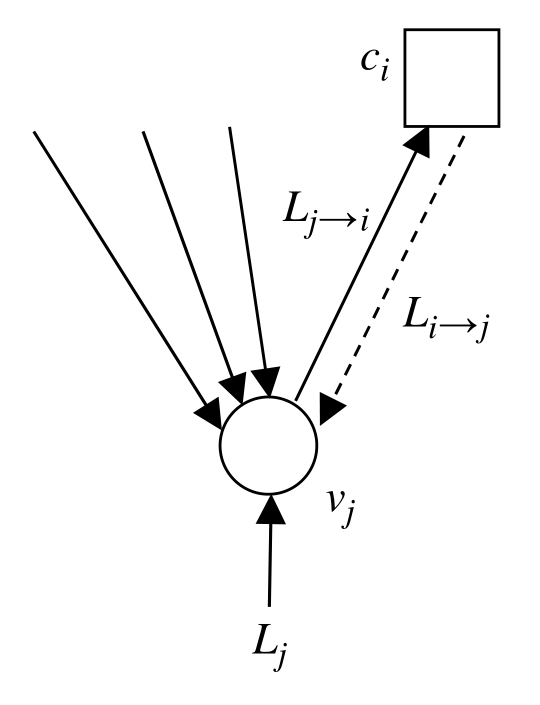
\includegraphics[width=0.9\textwidth]{figures/VN.png}
        \caption{Ο κόμβος \en{VN} $j$ (αποκωδικοποιητής \en{REP}) λαμβάνει πληροφορία από τους γειτονικούς \en{CN} (εκτός από τον $i$ $(L_{i\to j})$) και στέλνει στον \en{CN} $i$ την ποσότητα $L_{j\to i}$}
        \label{fig:VN}
    \end{minipage}\hfill
    \begin{minipage}{0.45\textwidth}
        \centering
        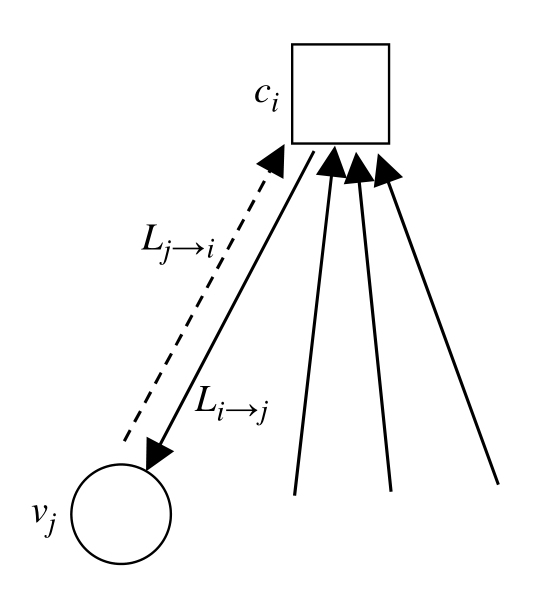
\includegraphics[width=0.9\textwidth]{figures/CN.png}
        \caption{Ο κόμβος \en{CN} $i$ (αποκωδικοποιητής \en{SPC}) λαμβάνει πληροφορία από τους γειτονικούς \en{VN} (εκτός από τον $j$ $(L_{j\to i})$) και στέλνει στον \en{VN} $j$ την ποσότητα $L_{i\to j}$}
        \label{fig:CN}
    \end{minipage}
\end{figure}

Οι αποκωδικοποιητές (κόμβοι) \en{VN} και \en{CN} λειτουργούν συνεργατικά για τον υπολογισμό της εκτίμησης $L(v_j|\mathbf{r}),\;\;j=0,1,\cdots,n-1$, επαναληπτικά. Κατά τη λειτουργία τους, υιοθετείται το \en{\textit{flooding schedule}}, σύμφωνα με το οποίο ξεκινώντας από τους \en{VN}, οι \en{VN} (\en{CN}) επεξεργάζονται την είσοδο και υπολογίζουν \textit{εξωγενή πληροφορία} την οποία στέλνουν στους γειτονικούς \en{CN} (\en{VN}). Η διαδικασία ολοκληρώνεται μετά από ένα προκαθορισμένο αριθμό επαναλήψεων ή αφού εκπληρωθεί ένα κριτήριο τερματισμού και υπολογίζεται η πιθανότητα $L(v_j|\mathbf{r})$, μέσω της οποίας λαμβάνεται απόφαση για την τιμή του \en{bit} $v_j$. Η υλοποίηση του \en{SPA} βασίζεται επίσης στη \textit{υπόθεση ανεξαρτησίας}: οι ληφθείσες ποσότητες \en{LLR} σε κάθε κόμβο από τους γειτονικούς, είναι μεταξύ τους ανεξάρτητες. Η υπόθεση αυτή, όμως, παύει να ισχύει από έναν αριθμό επαναλήψεων και μετά, γι\textquotesingle αυτό και ο \en{SPA} δεν εξάγει πάντα την ακριβή τιμή του $L(v_j|\mathbf{r})$ αλλά μια καλή προσέγγισή της.

Θα αναφερθούν επίσης οι εσωτερικές διαδικασίες και υπολογισμοί, που λαμβάνουν χώρα στους κόμβους \en{VN} και \en{CN}, για τον υπολογισμό της μετρικής \en{LLR} που ανταλλάσσεται μεταξύ γειτονικών κόμβων. Oι \en{VN} και \en{CN} λειτουργούν σαν \en{APP} επεξεργαστές για \en{REP} και \en{SPC} κώδικες αντίστοιχα, σε κάθε επανάληψη του αλγορίθμου.

Η εξωγενής πληροφορία που στέλνεται από τον \en{VN} $j$ στον \en{CN} $i$ δίνεται από την εξίσωση:

\begin{equation}
L_{j\to i} = L_j + \sum_{i'\in N(j)-\lbrace i\rbrace} L_{i'\to j}
\label{eq:CN update}
\end{equation}
, όπου η ποσότητα $L_j$ δίνεται από την εξίσωση \ref{eq:LLR}, αφού η ακολουθία $\mathbf{r}$ αντικατασταθεί από το κωδικό \en{bit} $r_j$. Η εξαίρεση του \en{i}-οστού \en{CN} κόμβου από το άθροισμα της Σχέσης \ref{eq:CN update} οφείλεται στην αρχή της εξωγενούς πληροφορίας: ένας κόμβος δεν παίρνει ξανά την πληροφορία που ο ίδιος είχε στείλει κατά το άλλο μισό της τρέχουσας επανάληψης. Αντίστοιχα, η εξωγενής πληροφορία που στέλνεται από τον \en{CN} $i$ στον \en{VN} $j$, δίνεται από την παρακάτω εξίσωση:

\begin{equation}
L_{i\to j} = 2\tanh^{-1} \left( \prod_{j'\in N(i)-\lbrace j\rbrace} \tanh \left( \frac{1}{2}L_{j'\to i} \right)\right)
\label{eq:VN update}
\end{equation}
, όπου και πάλι η εξαίρεση του \en{j}-οστού \en{VN} κόμβου οφείλεται στην αρχή της εξωγενούς πληροφορίας. Στο τέλος των επαναλήψεων, ο \en{VN} $j$ παράγει μια πρόβλεψη με βάση την ποσότητα

\begin{equation}
L_{j}^{total} = L_j + \sum_{i\in N(j)} L_{i\to j}
\label{eq:LLR total}
\end{equation}

Η πληροφορία $L_{j\to i}$ που ανταλάσσεται μεταξύ των \en{VN} $j$ και \en{CN} $i$, απoτελεί εκτίμηση της τιμής του $v_j$ (πρόσημο του $L_{j\to i}$) και το επίπεδο εμπιστοσύνης της τιμής (πλάτος του $L_{j\to i}$), βασισμένη στο \en{REP constraint} για τον αντίστοιχο κόμβο. Αντίστοιχα, η εκτίμηση του \en{CN} $i$ βασίζεται στο \en{SPC constraint}. Τέλος αναφέρεται πως για την αρχικοποίηση, χρησιμοποιείται η εξίσωση \ref{eq:LLR} με την τροποποίηση που αναφέραμε παραπάνω, η οποία διαμορφώνεται διαφορετικά για κάθε τύπο καναλιού. Ενδεικτικά, για το δυαδικό \en{AWGN} κανάλι, προκύπtει η σχέση:

\begin{equation}
L(v_j|r_j) = \frac{2r_j}{\sigma^2}
\label{eq:AWGN initial LLR}
\end{equation}

Τέλος, ο αλγόριθμος απαιτεί ένα κριτήριο τερματισμού. Χρησιμοποιείται η εξίσωση
\begin{equation*}
\mathbf{v}\mathbf{H}^T=\mathbf{0}
\end{equation*}
, όπου $\mathbf{v}$ είναι μια εκτίμηση της κωδικής λέξης στο πέρας κάθε επανάληψης \cite{ryan2009channel}, \cite{johnson2009iterative}, \cite{ta2013tutorial}.

\subsubsection{Ο \en{Sum-Product} αλγόριθμος για \en{RA}}

Αναφέρθηκε ήδη πως οι εξισώσεις \ref{eq:combiner equation} και \ref{eq:accumulator equation}, είναι οι εξισώσεις ελέγχου ισοτιμίας για ένα \en{RA} κώδικα. Η κωδικοποίηση είναι συστηματική, συνεπώς οι πρώτες $k$ στήλες του πίνακα $\mathbf{H}$ αντιστοιχούν στα \en{bits} πληροφορίας, ενώ οι επόμενες $m=n-k$ στήλες στα \en{parity bits}. Αναφέρθηκε επίσης πως ο πίνακας $m\times n \mathbf{H}$ είναι της μορφής

\begin{equation}
H=[H_1\;H_2]
\label{eq:RA parity check matrix form}
\end{equation}
όπου ο υποπίνακας $H_1$ είναι πίνακας $n-k\times k$ με βάρη γραμμών και στηλών, $(a,q)$ αντίστοιχα και ο $H_2$ οφείλεται στον συσσωρευτή.

Παρόμοια με τους \en{LDPC} κώδικες, το γράφημα \en{Tanner} των \en{RA} κωδίκων ορίζεται από τον πίνακα $\mathbf{H}$, με διαφορά ότι είναι εμφανής η διάκριση μεταξύ \en{info bits} και \en{parity bits}. Στο Σχήμα \ref{fig:RA tanner graph} φαίνεται το γράφημα \en{Tanner} ενός \en{RA}, στο οποίο γίνεται διάκριση μεταξύ των $k$ συστηματικών \en{bits} βαθμού $q$ στην κορυφή και των $m$ \en{parity bits} κόμβων βαθμού 2 (πλην του τελευταίου που διακρίνεται από βαθμό 1). Οι κόμβοι ελέγχου του γραφήματος διακρίνονται από βαθμό $a+2$, εκτός του τελευταίου που έχει βαθμό $a+1$ \cite{johnson2009iterative}.

\begin{figure}[H]
\center{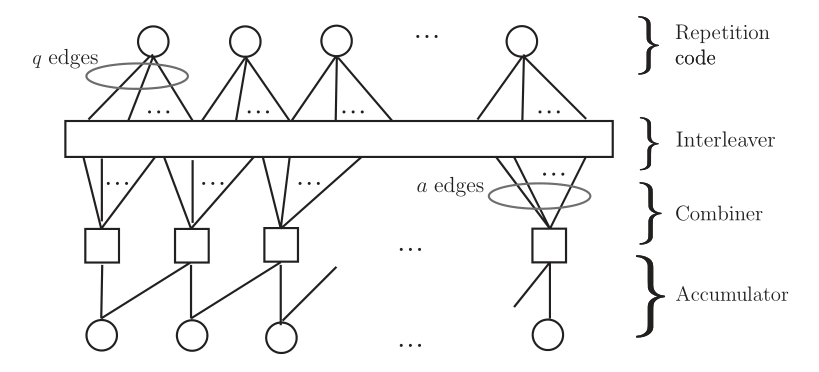
\includegraphics[width=0.85\linewidth]{figures/Ra_tanner.png}}
\caption{Γράφημα \en{Tanner RA} κώδικα}
\label{fig:RA tanner graph}
\end{figure}

Στην περίπτωση που οι κόμβοι \en{parity bits} και συστηματικών \en{bits} αντιμετωπίζονται ως ενιαίοι κόμβοι \en{bits} ο αλγόριθμος \en{SPA} για \en{RA} κώδικα, ταυτίζεται με αυτόν για ένα \en{LDPC} που έχει τον ίδιο πίνακα $\mathbf{H}$. Σε αντίθετη περίπτωση απαιτούνται τροποποιήσεις για τη συμπλήρωση μιας επανάληψης του αλγορίθμου.

Τέλος, ως σύγκριση μεταξύ του \en{Sum-Product} αποκωδικοποιητή και της \en{turbo} αποκωδικοποίησης, αναφέρεται πως, ενώ στον \en{SPA} οι \en{parity bit} κόμβοι αποκωδικοποιούνται όμοια με τους \en{systematic bit} κόμβους, ο \en{turbo} αποκωδικοποιητής χρησιμοποιεί \en{BCJR} αποκωδικοποιητή σε διάγραμμα \en{trellis}. Μέσω αυτού οι επαναλήψεις της \en{turbo} αποκωδικοποίησης είναι πιο πολύπλοκες, ωστόσο απαιτούνται λιγότερες επαναλήψεις συνολικά \cite{ryan2009channel}, \cite{johnson2009iterative}.
